%!TEX root = ../dissertation.tex
\begin{savequote}[75mm]
Nulla facilisi. In vel sem. Morbi id urna in diam dignissim feugiat. Proin molestie tortor eu velit. Aliquam erat volutpat. Nullam ultrices, diam tempus vulputate egestas, eros pede varius leo.
\qauthor{Quoteauthor Lastname}
\end{savequote}

\chapter{Experiments}
\label{ch:experiments}

\section{Barbara Experiments}

\label{sec:experimental}
We extended the MASON simulator to run our experiments.\cite{luke05mason}
We used the default parameters for the Flocking simulation that is included
with the MASON simulator, except without any randomness, cohesion, avoidance,
or dead agents.
% We received the code used to run Genter and Stone's experiments from them,
% but ultimately rewrote much of the influencing agent control code to handle
% our new settings and the distinction between local and global behaviors.
% and Stone to ensure that our implementations of their algorithms were similar.
% We do not describe those results here.
We sampled all metrics every $100$ time steps and ran all experiments for $100$
trials.

\subsection{No Influencing Agents}
Previous literature compared new influencing agent behaviors with baseline
influencing agent behaviors, but did not compare to settings with no
influencing agents.
In order to observe the marginal contribution of influencing agents
in future experiments, we start our investigation of the \textit{large} and
\textit{herd} settings by studying flock formation in those environments without
any influencing agents.
We use two metrics to evaluate flock formation: average number of flocks
formed and average proportion of lone agents at each time step.

In the \textit{large} setting , we test on a $1000x1000$ grid and vary the
number $N$ of Reynolds-Viscek agents from $50$ to $300$ in increments of $50$.
We run these simulations for $6000$ time steps.
In the \textit{herd} setting, we use a $5000x5000$ grid, position the herd in
the center of the grid with radius 500, and vary $N$ from $50$ to $300$ in
increments of $50$.
We run these simulations for $6000$ time steps.

\subsection{Influencing Agents in the Large Setting}
Next, we evaluate the contributions of influencing agents.
To evaluate the contributions of influencing agents in the \textit{large}
setting, we measure the time required for half of the Reynolds-Viscek agents
to face the same direction.
Unlike in previous work, which has limited the goal direction to a single
pre-determined goal direction, here we open up the possibility to convergence
to any direction to match the goal of our multi-step behavior.

We test the \textit{random}, \textit{grid}, and \textit{k-means} placement
strategies, along with global behaviors \textit{face}, \textit{random}, and
\textit{multistep}, each paired with local behaviors \textit{fact},
\textit{offset momentum}, \textit{one step lookahead}, and \textit{coordinated}.
We place $300$ Reynolds-Viscek agents on a $1000x1000$ grid, with $300$
Reynolds-Viscek agents and vary the number of influencing agents from $10$
to $100$ in intervals of $10$.

\subsection{Influencing Agents in the Herd Setting}
To evaluate the contributions of influencing agents in the \textit{herd} setting
we measure a slightly different metric.
Since we have two qualitatively different categories of global behaviors (net
behaviors vs. stationary behaviors), the number of agents facing the same
direction is irrelevant, since the stationary behaviors rotate the agents around
the origin (in fact, if the Reynolds-Viscek agents are all facing the same
goal direction, the stationary behavior has failed).
Instead, we measure the number of Reynolds-Viscek agents that are connected to
influencing agents at $15000$ time steps; at this point in time, all the agents
have travelled out of the grid, and no new interactions occur.
As a result, this is a measure of sustained influence over the Reynolds-Viscek
agents over time.

We examine the three circular placement strategies, \textit{circle-border},
\textit{circle-random}, and \textit{circle-grid}, with two placement radii,
\textit{500} and \textit{750}, along with the \textit{k-means} placement
strategy.
We split our examination of global behaviors between the \textit{net} behavior
(analogous to \textit{face}) and three stationary behaviors - namely
\textit{circle}, \textit{polygon}, and \textit{multicircle}.
We use a polygon with ten sides (a decagon) for our \textit{polygon} experiments,
and we vary the final radius for multicircle based on the initial placement
radius.
When the placement radius is \textit{500}, we set the final radius to
\textit{900}; when the placement radius is \textit{750}, we set the final radius
to \textit{1100}.
Finally, we pair the \textit{face}, \textit{offset momentum}, \textit{one step
lookahead}, and \textit{coordinated} local behaviors with all the global behaviors
and placement strategies.
We place $300$ Reynolds-Viscek agents inside a circle of radius $500$ at the center
of a $5000x5000$ grid, varying the number of influencing agents from $10$ to $100$
in intervals of $10$.

\section{Radhika Experiments}

NOTE: IN RADHIKA PAPER, EXPERIMENTS AND RESULTS WERE PRESENTED AT THE SAME TIME

\subsection{Evolutionary Experiments}
Each trial of one of the large-scale experiments takes dozens of seconds to run.
Furthermore, the random placement of the Reynolds-Viscek agents creates high
variability across multiple trials.
Consequently, using large-scale experiments to evaluate genomes during evolution
is infeasible.
Instead, we evaluate the genomes on a set of four small experiments, shown in
Figure $\ref{fig:evo}$.
\begin{figure}
    \centering
    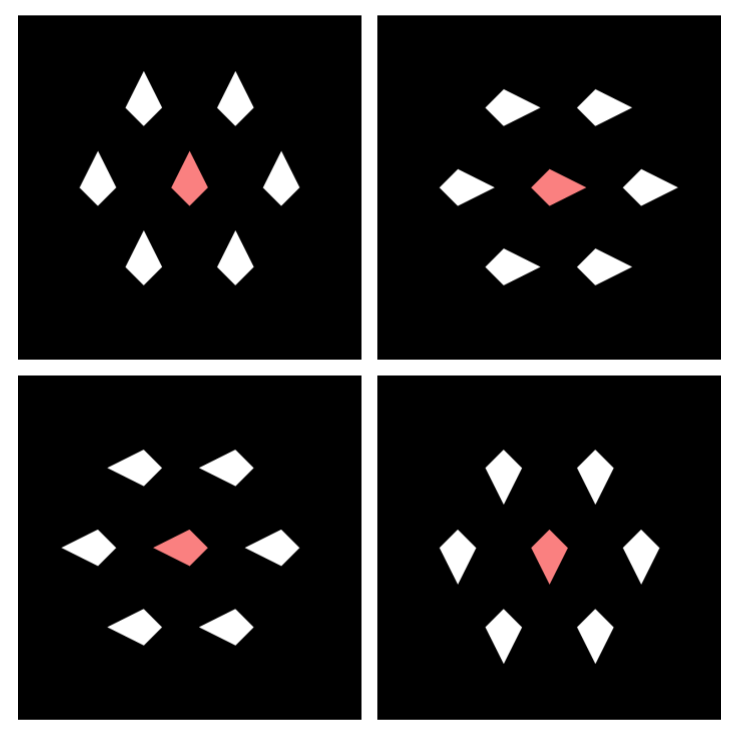
\includegraphics[width=0.45\textwidth]{evoall}
    \caption{The four starting positions we use to evaluate genomes during
    evolution.
    We run the simulation for $100$ steps and calculate the average angle offset
    from the goal direction across the six Reynolds-Viscek agents.
    The goal direction is east.}
    \label{fig:evo}
\end{figure}
In each of these experiments, the influencing agent is placed in the center of
six Reynolds-Viscek agents, each of which is at the edge of the influencing
agent's neighborhood.
All agents are initialized to face one of the cardinal directions, and we run
the simulation for $100$ steps.
At the end, we measure the average absolute angle difference, in degrees, from
the goal direction (east) across all six Reynolds-Viscek agents.
Lower values are better.
Initially, we evaluated genomes during evolution by randomly placing
Reynolds-Viscek agents in a circle around the influencing agent.
However, random placement resulted in high variability for the same genome
between generations, and it became difficult for the algorithm to find better
genomes.
We ultimately settled on a deterministic test to both reduce this variability
and to allow for memoization to make our algorithm run faster.

Finally, we add a small penalty for the number of nodes in the genome.
This gives the following cost function:
\[ \sum_{i=1}^6 \text{calcDiff}(\theta_i, \theta_{east}) + \alpha N_{nodes}, \]
where $N_{nodes}$ is the number of nodes in the genome, and $\alpha$ is a
regularization factor.
In our experiments, we set $\alpha=0.1$ to allow development of complexity but
to prevent blow-out.

\section{Genter and Stone experiments}
NEED TO PRESENT RESULTS FROM GENTER AND STONE EXPERIMENTS TOO
